\documentclass[11pt]{article}

    \usepackage[breakable]{tcolorbox}
    \usepackage{parskip} % Stop auto-indenting (to mimic markdown behaviour)
    
    \usepackage{iftex}
    \ifPDFTeX
    	\usepackage[T1]{fontenc}
    	\usepackage{mathpazo}
    \else
    	\usepackage{fontspec}
    \fi

    % Basic figure setup, for now with no caption control since it's done
    % automatically by Pandoc (which extracts ![](path) syntax from Markdown).
    \usepackage{graphicx}
    % Maintain compatibility with old templates. Remove in nbconvert 6.0
    \let\Oldincludegraphics\includegraphics
    % Ensure that by default, figures have no caption (until we provide a
    % proper Figure object with a Caption API and a way to capture that
    % in the conversion process - todo).
    \usepackage{caption}
    \DeclareCaptionFormat{nocaption}{}
    \captionsetup{format=nocaption,aboveskip=0pt,belowskip=0pt}

    \usepackage[Export]{adjustbox} % Used to constrain images to a maximum size
    \adjustboxset{max size={0.9\linewidth}{0.9\paperheight}}
    \usepackage{float}
    \floatplacement{figure}{H} % forces figures to be placed at the correct location
    \usepackage{xcolor} % Allow colors to be defined
    \usepackage{enumerate} % Needed for markdown enumerations to work
    \usepackage{geometry} % Used to adjust the document margins
    \usepackage{amsmath} % Equations
    \usepackage{amssymb} % Equations
    \usepackage{textcomp} % defines textquotesingle
    % Hack from http://tex.stackexchange.com/a/47451/13684:
    \AtBeginDocument{%
        \def\PYZsq{\textquotesingle}% Upright quotes in Pygmentized code
    }
    \usepackage{upquote} % Upright quotes for verbatim code
    \usepackage{eurosym} % defines \euro
    \usepackage[mathletters]{ucs} % Extended unicode (utf-8) support
    \usepackage{fancyvrb} % verbatim replacement that allows latex
    \usepackage{grffile} % extends the file name processing of package graphics 
                         % to support a larger range
    \makeatletter % fix for grffile with XeLaTeX
    \def\Gread@@xetex#1{%
      \IfFileExists{"\Gin@base"
.bb}%
      {\Gread@eps{\Gin@base.bb}}%
      {\Gread@@xetex@aux#1}%
    }
    \makeatother

    % The hyperref package gives us a pdf with properly built
    % internal navigation ('pdf bookmarks' for the table of contents,
    % internal cross-reference links, web links for URLs, etc.)
    \usepackage{hyperref}
    % The default LaTeX title has an obnoxious amount of whitespace. By default,
    % titling removes some of it. It also provides customization options.
    \usepackage{titling}
    \usepackage{longtable} % longtable support required by pandoc >1.10
    \usepackage{booktabs}  % table support for pandoc > 1.12.2
    \usepackage[inline]{enumitem} % IRkernel/repr support (it uses the enumerate* environment)
    \usepackage[normalem]{ulem} % ulem is needed to support strikethroughs (\sout)
                                % normalem makes italics be italics, not underlines
    \usepackage{mathrsfs}
    

    
    % Colors for the hyperref package
    \definecolor{urlcolor}{rgb}{0,.145,.698}
    \definecolor{linkcolor}{rgb}{.71,0.21,0.01}
    \definecolor{citecolor}{rgb}{.12,.54,.11}

    % ANSI colors
    \definecolor{ansi-black}{HTML}{3E424D}
    \definecolor{ansi-black-intense}{HTML}{282C36}
    \definecolor{ansi-red}{HTML}{E75C58}
    \definecolor{ansi-red-intense}{HTML}{B22B31}
    \definecolor{ansi-green}{HTML}{00A250}
    \definecolor{ansi-green-intense}{HTML}{007427}
    \definecolor{ansi-yellow}{HTML}{DDB62B}
    \definecolor{ansi-yellow-intense}{HTML}{B27D12}
    \definecolor{ansi-blue}{HTML}{208FFB}
    \definecolor{ansi-blue-intense}{HTML}{0065CA}
    \definecolor{ansi-magenta}{HTML}{D160C4}
    \definecolor{ansi-magenta-intense}{HTML}{A03196}
    \definecolor{ansi-cyan}{HTML}{60C6C8}
    \definecolor{ansi-cyan-intense}{HTML}{258F8F}
    \definecolor{ansi-white}{HTML}{C5C1B4}
    \definecolor{ansi-white-intense}{HTML}{A1A6B2}
    \definecolor{ansi-default-inverse-fg}{HTML}{FFFFFF}
    \definecolor{ansi-default-inverse-bg}{HTML}{000000}

    % commands and environments needed by pandoc snippets
    % extracted from the output of `pandoc -s`
    \providecommand{\tightlist}{%
      \setlength{\itemsep}{0pt}\setlength{\parskip}{0pt}}
    \DefineVerbatimEnvironment{Highlighting}{Verbatim}{commandchars=\\\{\}}
    % Add ',fontsize=\small' for more characters per line
    \newenvironment{Shaded}{}{}
    \newcommand{\KeywordTok}[1]{\textcolor[rgb]{0.00,0.44,0.13}{\textbf{{#1}}}}
    \newcommand{\DataTypeTok}[1]{\textcolor[rgb]{0.56,0.13,0.00}{{#1}}}
    \newcommand{\DecValTok}[1]{\textcolor[rgb]{0.25,0.63,0.44}{{#1}}}
    \newcommand{\BaseNTok}[1]{\textcolor[rgb]{0.25,0.63,0.44}{{#1}}}
    \newcommand{\FloatTok}[1]{\textcolor[rgb]{0.25,0.63,0.44}{{#1}}}
    \newcommand{\CharTok}[1]{\textcolor[rgb]{0.25,0.44,0.63}{{#1}}}
    \newcommand{\StringTok}[1]{\textcolor[rgb]{0.25,0.44,0.63}{{#1}}}
    \newcommand{\CommentTok}[1]{\textcolor[rgb]{0.38,0.63,0.69}{\textit{{#1}}}}
    \newcommand{\OtherTok}[1]{\textcolor[rgb]{0.00,0.44,0.13}{{#1}}}
    \newcommand{\AlertTok}[1]{\textcolor[rgb]{1.00,0.00,0.00}{\textbf{{#1}}}}
    \newcommand{\FunctionTok}[1]{\textcolor[rgb]{0.02,0.16,0.49}{{#1}}}
    \newcommand{\RegionMarkerTok}[1]{{#1}}
    \newcommand{\ErrorTok}[1]{\textcolor[rgb]{1.00,0.00,0.00}{\textbf{{#1}}}}
    \newcommand{\NormalTok}[1]{{#1}}
    
    % Additional commands for more recent versions of Pandoc
    \newcommand{\ConstantTok}[1]{\textcolor[rgb]{0.53,0.00,0.00}{{#1}}}
    \newcommand{\SpecialCharTok}[1]{\textcolor[rgb]{0.25,0.44,0.63}{{#1}}}
    \newcommand{\VerbatimStringTok}[1]{\textcolor[rgb]{0.25,0.44,0.63}{{#1}}}
    \newcommand{\SpecialStringTok}[1]{\textcolor[rgb]{0.73,0.40,0.53}{{#1}}}
    \newcommand{\ImportTok}[1]{{#1}}
    \newcommand{\DocumentationTok}[1]{\textcolor[rgb]{0.73,0.13,0.13}{\textit{{#1}}}}
    \newcommand{\AnnotationTok}[1]{\textcolor[rgb]{0.38,0.63,0.69}{\textbf{\textit{{#1}}}}}
    \newcommand{\CommentVarTok}[1]{\textcolor[rgb]{0.38,0.63,0.69}{\textbf{\textit{{#1}}}}}
    \newcommand{\VariableTok}[1]{\textcolor[rgb]{0.10,0.09,0.49}{{#1}}}
    \newcommand{\ControlFlowTok}[1]{\textcolor[rgb]{0.00,0.44,0.13}{\textbf{{#1}}}}
    \newcommand{\OperatorTok}[1]{\textcolor[rgb]{0.40,0.40,0.40}{{#1}}}
    \newcommand{\BuiltInTok}[1]{{#1}}
    \newcommand{\ExtensionTok}[1]{{#1}}
    \newcommand{\PreprocessorTok}[1]{\textcolor[rgb]{0.74,0.48,0.00}{{#1}}}
    \newcommand{\AttributeTok}[1]{\textcolor[rgb]{0.49,0.56,0.16}{{#1}}}
    \newcommand{\InformationTok}[1]{\textcolor[rgb]{0.38,0.63,0.69}{\textbf{\textit{{#1}}}}}
    \newcommand{\WarningTok}[1]{\textcolor[rgb]{0.38,0.63,0.69}{\textbf{\textit{{#1}}}}}
    
    
    % Define a nice break command that doesn't care if a line doesn't already
    % exist.
    \def\br{\hspace*{\fill} \\* }
    % Math Jax compatibility definitions
    \def\gt{>}
    \def\lt{<}
    \let\Oldtex\TeX
    \let\Oldlatex\LaTeX
    \renewcommand{\TeX}{\textrm{\Oldtex}}
    \renewcommand{\LaTeX}{\textrm{\Oldlatex}}
    % Document parameters
    % Document title
    \title{Home Exam HT2022}
    
    
    
    
    
% Pygments definitions
\makeatletter
\def\PY@reset{\let\PY@it=\relax \let\PY@bf=\relax%
    \let\PY@ul=\relax \let\PY@tc=\relax%
    \let\PY@bc=\relax \let\PY@ff=\relax}
\def\PY@tok#1{\csname PY@tok@#1\endcsname}
\def\PY@toks#1+{\ifx\relax#1\empty\else%
    \PY@tok{#1}\expandafter\PY@toks\fi}
\def\PY@do#1{\PY@bc{\PY@tc{\PY@ul{%
    \PY@it{\PY@bf{\PY@ff{#1}}}}}}}
\def\PY#1#2{\PY@reset\PY@toks#1+\relax+\PY@do{#2}}

\expandafter\def\csname PY@tok@w\endcsname{\def\PY@tc##1{\textcolor[rgb]{0.73,0.73,0.73}{##1}}}
\expandafter\def\csname PY@tok@c\endcsname{\let\PY@it=\textit\def\PY@tc##1{\textcolor[rgb]{0.25,0.50,0.50}{##1}}}
\expandafter\def\csname PY@tok@cp\endcsname{\def\PY@tc##1{\textcolor[rgb]{0.74,0.48,0.00}{##1}}}
\expandafter\def\csname PY@tok@k\endcsname{\let\PY@bf=\textbf\def\PY@tc##1{\textcolor[rgb]{0.00,0.50,0.00}{##1}}}
\expandafter\def\csname PY@tok@kp\endcsname{\def\PY@tc##1{\textcolor[rgb]{0.00,0.50,0.00}{##1}}}
\expandafter\def\csname PY@tok@kt\endcsname{\def\PY@tc##1{\textcolor[rgb]{0.69,0.00,0.25}{##1}}}
\expandafter\def\csname PY@tok@o\endcsname{\def\PY@tc##1{\textcolor[rgb]{0.40,0.40,0.40}{##1}}}
\expandafter\def\csname PY@tok@ow\endcsname{\let\PY@bf=\textbf\def\PY@tc##1{\textcolor[rgb]{0.67,0.13,1.00}{##1}}}
\expandafter\def\csname PY@tok@nb\endcsname{\def\PY@tc##1{\textcolor[rgb]{0.00,0.50,0.00}{##1}}}
\expandafter\def\csname PY@tok@nf\endcsname{\def\PY@tc##1{\textcolor[rgb]{0.00,0.00,1.00}{##1}}}
\expandafter\def\csname PY@tok@nc\endcsname{\let\PY@bf=\textbf\def\PY@tc##1{\textcolor[rgb]{0.00,0.00,1.00}{##1}}}
\expandafter\def\csname PY@tok@nn\endcsname{\let\PY@bf=\textbf\def\PY@tc##1{\textcolor[rgb]{0.00,0.00,1.00}{##1}}}
\expandafter\def\csname PY@tok@ne\endcsname{\let\PY@bf=\textbf\def\PY@tc##1{\textcolor[rgb]{0.82,0.25,0.23}{##1}}}
\expandafter\def\csname PY@tok@nv\endcsname{\def\PY@tc##1{\textcolor[rgb]{0.10,0.09,0.49}{##1}}}
\expandafter\def\csname PY@tok@no\endcsname{\def\PY@tc##1{\textcolor[rgb]{0.53,0.00,0.00}{##1}}}
\expandafter\def\csname PY@tok@nl\endcsname{\def\PY@tc##1{\textcolor[rgb]{0.63,0.63,0.00}{##1}}}
\expandafter\def\csname PY@tok@ni\endcsname{\let\PY@bf=\textbf\def\PY@tc##1{\textcolor[rgb]{0.60,0.60,0.60}{##1}}}
\expandafter\def\csname PY@tok@na\endcsname{\def\PY@tc##1{\textcolor[rgb]{0.49,0.56,0.16}{##1}}}
\expandafter\def\csname PY@tok@nt\endcsname{\let\PY@bf=\textbf\def\PY@tc##1{\textcolor[rgb]{0.00,0.50,0.00}{##1}}}
\expandafter\def\csname PY@tok@nd\endcsname{\def\PY@tc##1{\textcolor[rgb]{0.67,0.13,1.00}{##1}}}
\expandafter\def\csname PY@tok@s\endcsname{\def\PY@tc##1{\textcolor[rgb]{0.73,0.13,0.13}{##1}}}
\expandafter\def\csname PY@tok@sd\endcsname{\let\PY@it=\textit\def\PY@tc##1{\textcolor[rgb]{0.73,0.13,0.13}{##1}}}
\expandafter\def\csname PY@tok@si\endcsname{\let\PY@bf=\textbf\def\PY@tc##1{\textcolor[rgb]{0.73,0.40,0.53}{##1}}}
\expandafter\def\csname PY@tok@se\endcsname{\let\PY@bf=\textbf\def\PY@tc##1{\textcolor[rgb]{0.73,0.40,0.13}{##1}}}
\expandafter\def\csname PY@tok@sr\endcsname{\def\PY@tc##1{\textcolor[rgb]{0.73,0.40,0.53}{##1}}}
\expandafter\def\csname PY@tok@ss\endcsname{\def\PY@tc##1{\textcolor[rgb]{0.10,0.09,0.49}{##1}}}
\expandafter\def\csname PY@tok@sx\endcsname{\def\PY@tc##1{\textcolor[rgb]{0.00,0.50,0.00}{##1}}}
\expandafter\def\csname PY@tok@m\endcsname{\def\PY@tc##1{\textcolor[rgb]{0.40,0.40,0.40}{##1}}}
\expandafter\def\csname PY@tok@gh\endcsname{\let\PY@bf=\textbf\def\PY@tc##1{\textcolor[rgb]{0.00,0.00,0.50}{##1}}}
\expandafter\def\csname PY@tok@gu\endcsname{\let\PY@bf=\textbf\def\PY@tc##1{\textcolor[rgb]{0.50,0.00,0.50}{##1}}}
\expandafter\def\csname PY@tok@gd\endcsname{\def\PY@tc##1{\textcolor[rgb]{0.63,0.00,0.00}{##1}}}
\expandafter\def\csname PY@tok@gi\endcsname{\def\PY@tc##1{\textcolor[rgb]{0.00,0.63,0.00}{##1}}}
\expandafter\def\csname PY@tok@gr\endcsname{\def\PY@tc##1{\textcolor[rgb]{1.00,0.00,0.00}{##1}}}
\expandafter\def\csname PY@tok@ge\endcsname{\let\PY@it=\textit}
\expandafter\def\csname PY@tok@gs\endcsname{\let\PY@bf=\textbf}
\expandafter\def\csname PY@tok@gp\endcsname{\let\PY@bf=\textbf\def\PY@tc##1{\textcolor[rgb]{0.00,0.00,0.50}{##1}}}
\expandafter\def\csname PY@tok@go\endcsname{\def\PY@tc##1{\textcolor[rgb]{0.53,0.53,0.53}{##1}}}
\expandafter\def\csname PY@tok@gt\endcsname{\def\PY@tc##1{\textcolor[rgb]{0.00,0.27,0.87}{##1}}}
\expandafter\def\csname PY@tok@err\endcsname{\def\PY@bc##1{\setlength{\fboxsep}{0pt}\fcolorbox[rgb]{1.00,0.00,0.00}{1,1,1}{\strut ##1}}}
\expandafter\def\csname PY@tok@kc\endcsname{\let\PY@bf=\textbf\def\PY@tc##1{\textcolor[rgb]{0.00,0.50,0.00}{##1}}}
\expandafter\def\csname PY@tok@kd\endcsname{\let\PY@bf=\textbf\def\PY@tc##1{\textcolor[rgb]{0.00,0.50,0.00}{##1}}}
\expandafter\def\csname PY@tok@kn\endcsname{\let\PY@bf=\textbf\def\PY@tc##1{\textcolor[rgb]{0.00,0.50,0.00}{##1}}}
\expandafter\def\csname PY@tok@kr\endcsname{\let\PY@bf=\textbf\def\PY@tc##1{\textcolor[rgb]{0.00,0.50,0.00}{##1}}}
\expandafter\def\csname PY@tok@bp\endcsname{\def\PY@tc##1{\textcolor[rgb]{0.00,0.50,0.00}{##1}}}
\expandafter\def\csname PY@tok@fm\endcsname{\def\PY@tc##1{\textcolor[rgb]{0.00,0.00,1.00}{##1}}}
\expandafter\def\csname PY@tok@vc\endcsname{\def\PY@tc##1{\textcolor[rgb]{0.10,0.09,0.49}{##1}}}
\expandafter\def\csname PY@tok@vg\endcsname{\def\PY@tc##1{\textcolor[rgb]{0.10,0.09,0.49}{##1}}}
\expandafter\def\csname PY@tok@vi\endcsname{\def\PY@tc##1{\textcolor[rgb]{0.10,0.09,0.49}{##1}}}
\expandafter\def\csname PY@tok@vm\endcsname{\def\PY@tc##1{\textcolor[rgb]{0.10,0.09,0.49}{##1}}}
\expandafter\def\csname PY@tok@sa\endcsname{\def\PY@tc##1{\textcolor[rgb]{0.73,0.13,0.13}{##1}}}
\expandafter\def\csname PY@tok@sb\endcsname{\def\PY@tc##1{\textcolor[rgb]{0.73,0.13,0.13}{##1}}}
\expandafter\def\csname PY@tok@sc\endcsname{\def\PY@tc##1{\textcolor[rgb]{0.73,0.13,0.13}{##1}}}
\expandafter\def\csname PY@tok@dl\endcsname{\def\PY@tc##1{\textcolor[rgb]{0.73,0.13,0.13}{##1}}}
\expandafter\def\csname PY@tok@s2\endcsname{\def\PY@tc##1{\textcolor[rgb]{0.73,0.13,0.13}{##1}}}
\expandafter\def\csname PY@tok@sh\endcsname{\def\PY@tc##1{\textcolor[rgb]{0.73,0.13,0.13}{##1}}}
\expandafter\def\csname PY@tok@s1\endcsname{\def\PY@tc##1{\textcolor[rgb]{0.73,0.13,0.13}{##1}}}
\expandafter\def\csname PY@tok@mb\endcsname{\def\PY@tc##1{\textcolor[rgb]{0.40,0.40,0.40}{##1}}}
\expandafter\def\csname PY@tok@mf\endcsname{\def\PY@tc##1{\textcolor[rgb]{0.40,0.40,0.40}{##1}}}
\expandafter\def\csname PY@tok@mh\endcsname{\def\PY@tc##1{\textcolor[rgb]{0.40,0.40,0.40}{##1}}}
\expandafter\def\csname PY@tok@mi\endcsname{\def\PY@tc##1{\textcolor[rgb]{0.40,0.40,0.40}{##1}}}
\expandafter\def\csname PY@tok@il\endcsname{\def\PY@tc##1{\textcolor[rgb]{0.40,0.40,0.40}{##1}}}
\expandafter\def\csname PY@tok@mo\endcsname{\def\PY@tc##1{\textcolor[rgb]{0.40,0.40,0.40}{##1}}}
\expandafter\def\csname PY@tok@ch\endcsname{\let\PY@it=\textit\def\PY@tc##1{\textcolor[rgb]{0.25,0.50,0.50}{##1}}}
\expandafter\def\csname PY@tok@cm\endcsname{\let\PY@it=\textit\def\PY@tc##1{\textcolor[rgb]{0.25,0.50,0.50}{##1}}}
\expandafter\def\csname PY@tok@cpf\endcsname{\let\PY@it=\textit\def\PY@tc##1{\textcolor[rgb]{0.25,0.50,0.50}{##1}}}
\expandafter\def\csname PY@tok@c1\endcsname{\let\PY@it=\textit\def\PY@tc##1{\textcolor[rgb]{0.25,0.50,0.50}{##1}}}
\expandafter\def\csname PY@tok@cs\endcsname{\let\PY@it=\textit\def\PY@tc##1{\textcolor[rgb]{0.25,0.50,0.50}{##1}}}

\def\PYZbs{\char`\\}
\def\PYZus{\char`\_}
\def\PYZob{\char`\{}
\def\PYZcb{\char`\}}
\def\PYZca{\char`\^}
\def\PYZam{\char`\&}
\def\PYZlt{\char`\<}
\def\PYZgt{\char`\>}
\def\PYZsh{\char`\#}
\def\PYZpc{\char`\%}
\def\PYZdl{\char`\$}
\def\PYZhy{\char`\-}
\def\PYZsq{\char`\'}
\def\PYZdq{\char`\"}
\def\PYZti{\char`\~}
% for compatibility with earlier versions
\def\PYZat{@}
\def\PYZlb{[}
\def\PYZrb{]}
\makeatother


    % For linebreaks inside Verbatim environment from package fancyvrb. 
    \makeatletter
        \newbox\Wrappedcontinuationbox 
        \newbox\Wrappedvisiblespacebox 
        \newcommand*\Wrappedvisiblespace {\textcolor{red}{\textvisiblespace}} 
        \newcommand*\Wrappedcontinuationsymbol {\textcolor{red}{\llap{\tiny$\m@th\hookrightarrow$}}} 
        \newcommand*\Wrappedcontinuationindent {3ex } 
        \newcommand*\Wrappedafterbreak {\kern\Wrappedcontinuationindent\copy\Wrappedcontinuationbox} 
        % Take advantage of the already applied Pygments mark-up to insert 
        % potential linebreaks for TeX processing. 
        %        {, <, #, %, $, ' and ": go to next line. 
        %        _, }, ^, &, >, - and ~: stay at end of broken line. 
        % Use of \textquotesingle for straight quote. 
        \newcommand*\Wrappedbreaksatspecials {% 
            \def\PYGZus{\discretionary{\char`\_}{\Wrappedafterbreak}{\char`\_}}% 
            \def\PYGZob{\discretionary{}{\Wrappedafterbreak\char`\{}{\char`\{}}% 
            \def\PYGZcb{\discretionary{\char`\}}{\Wrappedafterbreak}{\char`\}}}% 
            \def\PYGZca{\discretionary{\char`\^}{\Wrappedafterbreak}{\char`\^}}% 
            \def\PYGZam{\discretionary{\char`\&}{\Wrappedafterbreak}{\char`\&}}% 
            \def\PYGZlt{\discretionary{}{\Wrappedafterbreak\char`\<}{\char`\<}}% 
            \def\PYGZgt{\discretionary{\char`\>}{\Wrappedafterbreak}{\char`\>}}% 
            \def\PYGZsh{\discretionary{}{\Wrappedafterbreak\char`\#}{\char`\#}}% 
            \def\PYGZpc{\discretionary{}{\Wrappedafterbreak\char`\%}{\char`\%}}% 
            \def\PYGZdl{\discretionary{}{\Wrappedafterbreak\char`\$}{\char`\$}}% 
            \def\PYGZhy{\discretionary{\char`\-}{\Wrappedafterbreak}{\char`\-}}% 
            \def\PYGZsq{\discretionary{}{\Wrappedafterbreak\textquotesingle}{\textquotesingle}}% 
            \def\PYGZdq{\discretionary{}{\Wrappedafterbreak\char`\"}{\char`\"}}% 
            \def\PYGZti{\discretionary{\char`\~}{\Wrappedafterbreak}{\char`\~}}% 
        } 
        % Some characters . , ; ? ! / are not pygmentized. 
        % This macro makes them "active" and they will insert potential linebreaks 
        \newcommand*\Wrappedbreaksatpunct {% 
            \lccode`\~`\.\lowercase{\def~}{\discretionary{\hbox{\char`\.}}{\Wrappedafterbreak}{\hbox{\char`\.}}}% 
            \lccode`\~`\,\lowercase{\def~}{\discretionary{\hbox{\char`\,}}{\Wrappedafterbreak}{\hbox{\char`\,}}}% 
            \lccode`\~`\;\lowercase{\def~}{\discretionary{\hbox{\char`\;}}{\Wrappedafterbreak}{\hbox{\char`\;}}}% 
            \lccode`\~`\:\lowercase{\def~}{\discretionary{\hbox{\char`\:}}{\Wrappedafterbreak}{\hbox{\char`\:}}}% 
            \lccode`\~`\?\lowercase{\def~}{\discretionary{\hbox{\char`\?}}{\Wrappedafterbreak}{\hbox{\char`\?}}}% 
            \lccode`\~`\!\lowercase{\def~}{\discretionary{\hbox{\char`\!}}{\Wrappedafterbreak}{\hbox{\char`\!}}}% 
            \lccode`\~`\/\lowercase{\def~}{\discretionary{\hbox{\char`\/}}{\Wrappedafterbreak}{\hbox{\char`\/}}}% 
            \catcode`\.\active
            \catcode`\,\active 
            \catcode`\;\active
            \catcode`\:\active
            \catcode`\?\active
            \catcode`\!\active
            \catcode`\/\active 
            \lccode`\~`\~ 	
        }
    \makeatother

    \let\OriginalVerbatim=\Verbatim
    \makeatletter
    \renewcommand{\Verbatim}[1][1]{%
        %\parskip\z@skip
        \sbox\Wrappedcontinuationbox {\Wrappedcontinuationsymbol}%
        \sbox\Wrappedvisiblespacebox {\FV@SetupFont\Wrappedvisiblespace}%
        \def\FancyVerbFormatLine ##1{\hsize\linewidth
            \vtop{\raggedright\hyphenpenalty\z@\exhyphenpenalty\z@
                \doublehyphendemerits\z@\finalhyphendemerits\z@
                \strut ##1\strut}%
        }%
        % If the linebreak is at a space, the latter will be displayed as visible
        % space at end of first line, and a continuation symbol starts next line.
        % Stretch/shrink are however usually zero for typewriter font.
        \def\FV@Space {%
            \nobreak\hskip\z@ plus\fontdimen3\font minus\fontdimen4\font
            \discretionary{\copy\Wrappedvisiblespacebox}{\Wrappedafterbreak}
            {\kern\fontdimen2\font}%
        }%
        
        % Allow breaks at special characters using \PYG... macros.
        \Wrappedbreaksatspecials
        % Breaks at punctuation characters . , ; ? ! and / need catcode=\active 	
        \OriginalVerbatim[#1,codes*=\Wrappedbreaksatpunct]%
    }
    \makeatother

    % Exact colors from NB
    \definecolor{incolor}{HTML}{303F9F}
    \definecolor{outcolor}{HTML}{D84315}
    \definecolor{cellborder}{HTML}{CFCFCF}
    \definecolor{cellbackground}{HTML}{F7F7F7}
    
    % prompt
    \makeatletter
    \newcommand{\boxspacing}{\kern\kvtcb@left@rule\kern\kvtcb@boxsep}
    \makeatother
    \newcommand{\prompt}[4]{
        \ttfamily\llap{{\color{#2}[#3]:\hspace{3pt}#4}}\vspace{-\baselineskip}
    }
    

    
    % Prevent overflowing lines due to hard-to-break entities
    \sloppy 
    % Setup hyperref package
    \hypersetup{
      breaklinks=true,  % so long urls are correctly broken across lines
      colorlinks=true,
      urlcolor=urlcolor,
      linkcolor=linkcolor,
      citecolor=citecolor,
      }
    % Slightly bigger margins than the latex defaults
    
    \geometry{verbose,tmargin=1in,bmargin=1in,lmargin=1in,rmargin=1in}
    
    

\begin{document}
    
    \maketitle
    
    

    
    \hypertarget{gmi26h-cryptography-home-exam}{%
\section{GMI26H Cryptography Home
Exam}\label{gmi26h-cryptography-home-exam}}

    P1 HT22, Dalarna University

\begin{enumerate}
\def\labelenumi{(\alph{enumi})}
\setcounter{enumi}{2}
\tightlist
\item
  Joonas Pääkkönen
\end{enumerate}

\hypertarget{this-is-the-final-version-of-the-home-exam.-we-will-not-be-adding-any-more-questions.}{%
\subsection{This is the final version of the home exam. We will not be
adding any more
questions.}\label{this-is-the-final-version-of-the-home-exam.-we-will-not-be-adding-any-more-questions.}}

\hypertarget{questions-13-to-24-are-short-questions-that-must-be-answered-with-just-a-couple-of-sentences-with-or-without-a-single-optional-figure.-references-are-not-required-for-these-answers.-be-concise-and-on-point.}{%
\subsubsection{Questions 13 to 24 are ``short questions'' that must be
answered with just a couple of sentences with or without a single
optional figure. References are not required for these answers. Be
concise and on
point.}\label{questions-13-to-24-are-short-questions-that-must-be-answered-with-just-a-couple-of-sentences-with-or-without-a-single-optional-figure.-references-are-not-required-for-these-answers.-be-concise-and-on-point.}}

\hypertarget{you-may-write-your-answers-in-english-or-swedish}{%
\subsubsection{You may write your answers in English or
Swedish}\label{you-may-write-your-answers-in-english-or-swedish}}

Remember that the Links folder in Learn may include useful links

Knowing LaTeX is not a requirement but it may make the few equations
that may be needed in your answers prettier, e.g.~you may write
``\(a^2 = b \mod 3\)'' instead of ``a\^{}2 = b mod 3''

\hypertarget{use-file---download-as-or-print-to-pdf-in-browser-to-download-this-file-with-your-answers-as-.pdf-and-you-will-see-the-length-of-each-answer-in-.pdf-format}{%
\subsubsection{Use ``File -\textgreater{} Download as'' or ``Print to
PDF'' in browser to download this file (with your answers) as .pdf and
you will see the length of each answer in .pdf
format}\label{use-file---download-as-or-print-to-pdf-in-browser-to-download-this-file-with-your-answers-as-.pdf-and-you-will-see-the-length-of-each-answer-in-.pdf-format}}

\hypertarget{deadline-for-the-entire-home-exam-thursday-october-27th-at-1159-pm}{%
\subsubsection{Deadline for the entire home exam: Thursday October 27th
at 11:59
PM}\label{deadline-for-the-entire-home-exam-thursday-october-27th-at-1159-pm}}

Home exam submission folder will be opened later (some days before the
deadline)

The maximum length of an essay is 2 pages .pdf format. If your essay
contains one or more images or plots, the maximum is 2.5 pages.

    The following information is directly from the study guide:

Home exam: One written home exam which is orally examined. Essays,
terminology and short Python exercises. See the notes in the preface of
the home exam. The maximum length of an essay is 2 pages .pdf format. If
your essay contains one or more images or plots, the maximum is 2.5
pages.

The written home exam will be updated approximately once a week so it is
published in multiple parts. More questions will be added in each part.
At the oral exam of the home exam, any part of the home exam may be
examined. All parts of the home exam need to be submitted in one long
JNB .ipynb file as well as in .pdf. There will be no (extensive)
mathematics in the home exam, apart from perhaps a short formula here or
there, but understanding the basics of the mathematics behind
cryptography will surely improve your general understanding of the
algorithms. Python and Sage can be used to add plots, diagrams and
flowcharts to JNB files. You can also add your own drawings to your
answers by taking pictures and using the Insert Image command in
Markdown cells.

You must be able to answer the questions in the oral exam of the home
exam without looking at the written answers, though this does not mean
that you cannot share your screen. However, if all you can do is to read
every answer from your screen word for word, it's a telltale sign that
you have not understood the concept and may have simply copy-pasted your
answers from somewhere else.

If you have included a drawing or any other figure in your solutions,
please do share your screen in the oral exam of the home exam and
explain the drawing. You may also have a drawing app open on your
computer and draw or write additional things on the fly, if you want.

Students are encouraged to discuss cryptography at a general level with
fellow students, though each student must write and submit his or her
own solutions to the home exam and the AES project. Remember that on
Learn you can look for everyone's username (and thus email address
handle) under ``Roster → View everyone in your course'' so you can email
and ask others if you are looking for study buddies. The home exam is
individual with individual solutions but working with fellow students is
not prohibited. However, if you work with a fellow student, you must
mention who you worked with in your answers. For instance: ``On
questions 2 and 4, I was working together with Carin Keysson''.

Also remember that it is usually good practice to refer to several
sources of information, not only one (e.g.~always only a Wikipedia
article).

Presentations (oral exams): The AES project and the home exam will be
orally presented. During your AES presentation we will look at your code
and answers together and you will be asked questions regarding your
implementation. You must be able to explain how your code works. If you
have had help from others you must comment this in your code. You must
comment if you have discussed your code or collaborated with fellow
students and comment this for every class/method and give credit to the
right person. The same goes if you have looked at code from the
internet.

Bring a valid ID card (e.g.~a driver's license or a DU access card with
a picture) to each of the oral exams.

Submissions: Students are encouraged to discuss the labs with fellow
students, but everything must be submitted personally on Learn. Each
student must write and submit individual solutions.

Resubmissions: The home exam written exam and the AES project can be
resubmitted twice until the student passes them. Also the oral exams can
be retaken twice.

Plagiarism: Uphold academic integrity and honesty. Do not plagiarise.
Plagiarism means that your text or code reproduces the contents of
someone else's text or code without referencing to the original text or
code. Plagiarism can at worst lead to suspension from studies and
instructors are required to report all discovered plagiarism. To avoid
plagiarism, it is important that students learn how to quote and cite
correctly. Do not submit answers written by other students.

Week 43: last week before exam week, one deadline for both home exam
written exam and AES report: Thursday October 27th at 11:59 PM (Thursday
night before the exam week)

Week 44: exam week, reserved Monday morning + Tuesday morning for AES
oral exams, whole Friday for home exam oral exams. Exact times of
individual oral exams are TBA.

\hypertarget{questions-up-to-question-2424.}{%
\subsubsection{Questions up to question
24/24.}\label{questions-up-to-question-2424.}}

    \hypertarget{question-1}{%
\subsection{Question 1*:}\label{question-1}}

(essay, max length 2.5 pages including figures)

Essay title: Explain the Transport Layer Security (TLS) protocol

Especially focus on the latest version 1.3 and the cryptographic aspects
of the protocol. Especially pay attention to the related terminology and
concepts covered in the course.

Your essay needs to define and include the concept of ``cipher suite''
and discuss the cipher suite used in TLS.

You may also visit e.g.~your favourite websites and see if they are
using TLS (and what version, 1.3 maybe) for encryption and
authentication.

*This question has been turned into a bonus question. It is not
compulsory to answer this question but answering it well makes your
overall home exam stronger.

    \hypertarget{question-2}{%
\subsection{Question 2:}\label{question-2}}

(essay, max length 2.5 pages including figures)

Essay title: Next Generation Encryption (NGE)

Discuss Next Generation Encryption (NGE) especially from the point of
view of the algorithms discussed in the course and e.g.~the recommended
key lengths for these algorithms

    \hypertarget{next-generation-encryption}{%
\subsection{Next Generation
Encryption}\label{next-generation-encryption}}

Encryption has existed for millennia now; a rather famous example is the
Caesar cipher, which is a rather simple substitution cipher that shifts
each letter of the alphabet by a given number. As an example, if the if
it's a right shift of 5 then A becomes F and X would become B (``Caesar
cipher'', 2022). In the 16th century the first encryption scheme using a
key was introduced, 19th century introduced the Playfair cipher which
encrypted pairs of letters instead of single letters. But it wasn't
until the second world war where encryption, and decryption, played and
integral part in the allied victory. Alan Turing managed to break the
Enigma machine used by the Germans. Ever seen then the usage of
encryption has exploded, virtually all data today is encrypted (Thales
group, 2021). This essay will focus on what encryption methods are used
today, but more crucially how the future will affect these algorithms
and what the future looks like for encryption.

DES, in full Data Encryption Standard, is a symmetric-key encryption
algorithm. Symmetric encryption means that the same key is used for both
encryption and decryption. The encryption standard was approved in 1976
but it was officially replaced by AES in 2002 (``Data Encryption
Standard'', 2022). DES has no inherent design flaws but is no longer
considered secure as the key size is way too small and can easily be
brute forced by the computational power that is available today. AES,
for example, uses both 128 and 256-bit keys while DES is stuck using
56-bit keys. DES also has problems where it is only efficient in
hardware implementations but not software implementations, standards
have changed, and DES is no longer seen as being adequate in both
performance and security (Saha, 2022).

3DES, also called triple-DES, works the same as DES but utilizes three
keys instead of just one. Since each key in DES is 56-bit, this means
that 3DES combined can give security of 112 or 168 bits, 3DES applies
the DES algorithm three times to each block (``Triple DES'', 2022). 3DES
was introduced in 1999 as an alternative to DES, it was a convenient as
it could utilize existing equipment and infrastructure, but it is now
going to be disallowed to be used in new applications after 2023 (Saha,
2022). This is partially due to a vulnerability being found, the limited
block size of 3DES opens the potential for a birthday attack. It's an
attack where if you send enough traffic to cause a collision it is
possible to recover information such as a session cookie (Salz, 2016).

RSA, named after the creators Rivest-Shamir-Adleman, is one of the
oldest public-key cryptosystems. This system utilizes a public
encryption key and a private decryption key, the encryption key is based
on two large prime numbers. This means that anyone can encrypt a message
but only the person with the two secret prime numbers is able to decrypt
the messages (``RSA (cryptosystem)'', 2022). RSA is still used today and
is still considered secure for the tasks that it is generally used for,
provided you know the weaknesses and apply it correctly. Recommended
minimum key size is 2048 bits but 4096-bit keys are used when dealing
with sensitive information. One problem that will be problematic in the
future is quantum computing, this will most likely require a change in
RSA or a completely new system (Lake, 2021).

Stallings (2022) uses the term ``post-quantum cryptography'' to describe
how future cryptography algorithms need to be designed to be secure
against the potential future of quantum computers. Currently no
organization is using a post-quantum safe cryptographic algorithm, DES
and 3DES are already discontinued or about to be but RSA is expected to
no longer be secure in a post-quantum cryptography (Stallings, 2022).
Public-key cryptography is already proven to be broken by quantum
computing by using ``Shor's algorithm'' (2022). Out of the ones
mentioned before the only one expected to survive quantum computing is
AES, which is symmetric encryption, is expected to be quantum resistant
as it can take a key size of 256 bits. According to Grover's algorithm
AES-256 in a post-quantum world should have the same security as AES-128
has today (Wagner, 2020).

Quantum computers are getting faster and faster by the year, and while
it has many problems to overcome, it is considered a very real
possibility (William, 2021). There have already been alternatives
announced and more are on their way getting developed right now as
stated by NIST (2022), there will always a race between cryptography and
computational power. Q-day is a term coined to describe the day that
quantum computers hit the internet, almost everything on the internet is
made possible by cryptographic algorithms. Q-day stands to threaten the
operation of the internet if nothing is done in time. Therefore, the
search for quantum safe cryptographic algorithms is one of the most
important ones (Castelvecchi, 2022).  

References

Wikipedia contributors. (2022, October 13). Caesar cipher. In Wikipedia,
The Free Encyclopedia. Retrieved 16:12, October 19, 2022, from
https://en.wikipedia.org/w/index.php?title=Caesar\_cipher\&oldid=1115923163

Thales group. (2021, October 1). A brief history of encryption (and
cryptography).
https://www.thalesgroup.com/en/markets/digital-identity-and-security/magazine/brief-history-encryption

Wikipedia contributors. (2022, August 7). Data Encryption Standard. In
Wikipedia, The Free Encyclopedia. Retrieved 16:30, October 19, 2022,
from
https://en.wikipedia.org/w/index.php?title=Data\_Encryption\_Standard\&oldid=1102983038

Saha, P. (2022, March 26). Why 3DES or Triple DES is Officially Being
Retired.
https://www.encryptionconsulting.com/why-3des-or-triple-des-is-officially-being-retired/

Wikipedia contributors. (2022, September 27). Triple DES. In Wikipedia,
The Free Encyclopedia. Retrieved 17:15, October 19, 2022, from
https://en.wikipedia.org/w/index.php?title=Triple\_DES\&oldid=1112642613

Bhandari, S. (2022, October 7). Difference between AES and 3DES.
https://askanydifference.com/difference-between-aes-and-3des/

Salz, R. (2016, August 24). The SWEET32 Issue, CVE-2016-2183
https://www.openssl.org/blog/blog/2016/08/24/sweet32/

Wikipedia contributors. (2022, October 25). RSA (cryptosystem). In
Wikipedia, The Free Encyclopedia. Retrieved 17:57, October 19, 2022,
from
https://en.wikipedia.org/w/index.php?title=RSA\_(cryptosystem)\&oldid=1118240043

Lake, J. (2021, March 18). What is RSA encryption and how does it work?.
https://www.comparitech.com/blog/information-security/rsa-encryption/

Stallings, W. (2022). Cryptography and Network Security: Principles and
Practice. Pearson.

Wikipedia contributors. (2022, October 5). Shor's algorithm. In
Wikipedia, The Free Encyclopedia. Retrieved 23:31, October 20, 2022,
from
https://en.wikipedia.org/w/index.php?title=Shor\%27s\_algorithm\&oldid=1114153732

Wagner, L. (2020, September 10). Is AES-256 Quantum Resistant?.
https://medium.com/bootdotdev/is-aes-256-quantum-resistant-4dc3447e7b82

Williams, A. (2021, March 11). How close are we to a quantum future?.
https://medium.com/one-pale-blue-dot/how-close-are-we-to-a-quantum-future-6abb38f551f7

NIST. (2022, July 5). NIST Announces First Four Quantum-Resistant
Cryptographic Algorithms.
https://www.nist.gov/news-events/news/2022/07/nist-announces-first-four-quantum-resistant-cryptographic-algorithms

Castelvecchi, D. (2022, February 8). The race to save the Internet from
quantum hackers. https://www.nature.com/articles/d41586-022-00339-5

    \hypertarget{question-3}{%
\subsection{Question 3:}\label{question-3}}

(essay, max length 2.5 pages including figures)

Essay title: Cryptographic security services

Several security services may be provided using cryptographic
mechanisms. Such services include confidentiality, data integrity,
authentication, authorization and non-repudiation. Often a combination
of these services is required.

Discuss these security services especially from the point of view of the
algorithms discussed in the course, what they mean (definitions of
confidentiality, data integrity, authentication, authorization and
non-repudiation must be included) and what cryptographic mechanisms or
algorithms can be used to achieve them.

    \hypertarget{cryptographic-security-services}{%
\subsection{Cryptographic security
services}\label{cryptographic-security-services}}

The goal of information security is to protect information, by
preventing or reducing the risk of data getting into the wrong hands.
The challenges that come with information security are varied by it can
be summarized by balancing confidentiality, integrity, and availability
of data (``Information security'', 2022). This is called the CIA triad;
confidentiality is the assurance that the data remains hidden. Integrity
is about making sure that the data can be trusted and has not been
altered, availability is the idea that the data is useless if you are
not able to access it when you need to (Fortinet, n.d.). There are many
more concepts or services which are a part of what will be explored in
this essay, we will also look at what cryptographic algorithms or
mechanisms that are used to make these ideas possible.

Confidentiality, as stated previously, is making sure that data stays
hidden. A strong cryptographic algorithm such as AES-256 ensures that
the data is secured even if they have access to the ciphertext, AES-256
is considered very hard to break which means that the actual information
contained is kept a secret (``Advanced Encryption Standard'',2022).
Integrity is provided using checksums, a checksum is a piece of
information that is used to verify that the data stays the same. There
are various ways of generating checksums, but we will focus on the
cryptographic hash functions which generate checksums with extra
cryptographic properties. Among these properties are things like making
sure it's one way, meaning that you cannot extract the data from the
checksum, there is also the idea of diffusion which means that the
checksum should change greatly even if there are small changes in the
data (Versity, 2018). Availability is important but not necessarily
provided by cryptography and we will therefore not go more in-depth.

Authentication is making sure that the users are who they say they are,
this is especially useful if you want to stop a man-in-the-middle
attack. This attack allows a user to act as a middleman and can
potentially send malicious messages or information (``Authentication'',
2022). Cryptographic authentication is a way to identify the user by
making them prove that they possess their private key (Pomcor, n.d.). A
digital signature is used in key-based authentication where a user
requests information, the server generates a value and sends it to the
user and the user the uses their private key to create a digital
signature and uses that to check if the user is who they claim to be. It
is important that the keys stay private as anyone with access to the key
can use it to make maliciously (Garantir, 2022).

Authorization is verifying if the user has permission to use or access a
piece of data. Authorization and authentication are usually combined
since authentication makes sure that the user is who they say they are
while authorization checks what permissions the user has (Information
Services \& Technology, n.d.). This is often paired with or called
access control, by for example using access control lists you can
compare the user to an access control list to give them the permission
to access or edit files (IBM, 2021).

Non-repudiation is the idea that a user cannot deny the authenticity of
data, more specifically in digital security non-repudiation is provided
when proof of integrity and the origin of data is provided, high
confidence in authentication and that the data is available when it
should be (``Non-repudiation'', 2022). As an example, digital signatures
can be used if a user wants to purchase a product online. A digital
signature requires the user to ``sign'' using their private key, if this
user has kept their private key secure this would then provide some
confidence in the authenticity. This combined with other measures
provide non-repudiation (Cryptomathic, n.d.).

The point of the essay was to show what services are considered
important and how these are provided using cryptography. We have
identified key concepts and services, we identified how these can be
provided in a service using cryptographic mechanisms such as digital
signatures, cryptographic algorithms, and access control.

Reference 

Wikipedia contributors. (2022, October 24). Information security. In
Wikipedia, The Free Encyclopedia. Retrieved 01:06, October 16, 2022,
from
https://en.wikipedia.org/w/index.php?title=Information\_security\&oldid=1117886931

Fortinet. (n.d.). CIA Triad.
https://www.fortinet.com/resources/cyberglossary/cia-triad

Wikipedia contributors. (2022, October 22). Advanced Encryption
Standard. In Wikipedia, The Free Encyclopedia. Retrieved 01:39, October
16, 2022, from
https://en.wikipedia.org/w/index.php?title=Advanced\_Encryption\_Standard\&oldid=1117488157

Versity. (2018, August 21). Data Integrity Checksums.
https://www.versity.com/data-integrity-checksums/

Wikipedia contributors. (2022, October 16). Authentication. In
Wikipedia, The Free Encyclopedia. Retrieved 02:16, October 16, 2022,
from
https://en.wikipedia.org/w/index.php?title=Authentication\&oldid=1116332126

Pomcor. (n.d.). Cryptographic Authentication for Web Applications.
https://pomcor.com/cryptographic-authentication/

Garantir. (2021, August 17). Key-Based Authentication: Using
Cryptographic Controls To Manage Access To Enterprise Resources.
https://garantir.io/key-based-authentication/

Information Services \& Technology. (n.d.). Understanding
Authentication, Authorization, and Encryption.
https://www.bu.edu/tech/about/security-resources/bestpractice/auth/

Wikipedia contributors. (2022, August 26). Non-repudiation. In
Wikipedia, The Free Encyclopedia. Retrieved 16:14, October 16, 2022,
from
https://en.wikipedia.org/w/index.php?title=Non-repudiation\&oldid=1106835323

IBM. (2021, March 4). Authentication versus access control.
https://www.ibm.com/docs/en/wca/3.0.0?topic=security-authentication-versus-access-control

Cryptomathic. (n.d.). What is non-repudiation?.
https://www.cryptomathic.com/products/authentication-signing/digital-signatures-faqs/what-is-non-repudiation

    \hypertarget{question-4}{%
\subsection{Question 4:}\label{question-4}}

(essay, max length 2.5 pages including figures)

Essay title: Data Encryption Standard (DES)

Data Encryption Standard (DES) is a famous Feistel cipher. Start by
explaining the Feistel cipher, what it is and what makes it a good
cryptographic mechanism and how DES is built upon it. However, the
original DES is nowadays considered insecure, and instead, Triple DES is
recommended. Explain why DES is considered insecure, what Triple DES is
and how it improves on the original DES.

    \hypertarget{data-encryption-standard}{%
\subsection{Data Encryption Standard}\label{data-encryption-standard}}

DES, in full Data Encryption Standard, is a symmetric-key encryption
algorithm which was used for the encryption of digital data. DES is
based on the Feistel cipher, the cipher divides the plaintext in half
leading to two blocks. It then uses rounds where it's first a
substitution step and a permutation step (``Data Encryption Standard'',
2022). The Feistel cipher is a good basis for an encryption algorithm
because it blends confusion and diffusion, and the idea about the ideal
block cipher. As already described confusion and diffusion is provided
by the substitution and permutation steps in the algorithm, confusion
simply put is the idea that each bit should be dependent on multiple
parts of the key and diffusion means that if we change a bit roughly
half the bits should change. The ideal block cipher is the idea that the
relationship between the input block and out block should be completely
random, but must be invertible (Stallings, 2022).

DES is just an example of a Feistel cipher, the Feistel cipher is a
model for which many ciphers are based on. DES has the same structure as
a Feistel cipher, with exception for the first and final permutations.
Being a Feistel cipher means that it uses the same algorithm for both
encryption and decryption (Tutorialspoint, n.d.). Since the structure is
the same, both Feistel and DES alternates substitution and permutation.
The Feistel structure is based on the structure Shannon proposed in
1945. Shannon showed how the ideas of confusion and diffusion could be
achieved in encryption. Even if an attacker knows the encryption
algorithm, they should not be able to decipher the ciphertext without
knowing the key (Tokenex, n.d.). This idea is called the ``Kerckhoffs's
principle'' (2022), the system should be secure even if everything
except for the key is publicly known.

The problem with DES in today's world is that computational power has
risen a lot and the key size of DES is way too small for today's usage.
Generally, a bigger key is considered safer as brute forcing takes a lot
longer. At the time of the introduction of DES computers that could go
over the whole key domain were very expensive but as computational power
has gone up the security has gone down for DES (Ginni, 2022). There are
no inherent flaws in the design of DES, but it is considered out of date
because of the key size. This is where 3DES, also called triple-DES,
comes in. 3DES addresses the key length weakness of DES. DES uses a key
size of 56 bits while 3DES uses three different keys of the same length,
56 bits. The essentially results in a 168-bit key which is significantly
more secure than 56 bits. Interestingly 3DES is falling out of fashion
as it is not seen as secure anymore but that is past the scope of this
essay (Saha, 2022).

As demand for better encryption standards grew with the rising
computational power, 3DES filled a special spot as it was possible to
utilize existing equipment and infrastructure previously used by DES.
The problem that 3DES had is that, while it is safer, it is also a lot
slower. When compared to AES, 3DES performs much worse and as expected
it is substantially slower when compared to DES. NIST, in full National
Institute of Standards and Technology, said that the DES replacement had
to be perform efficiently in both hardware and software implementations.
A major problem with DES in this regard is that it was only efficient in
hardware implementations (Townsend security, 2021).

As we approach the end of an era, DES has already gone out of use and
3DES will probably go out of use in 2023/2024. While they are quite
resistant to cryptanalysis and have no known major design flaws, it is
important to remember that no encryption standard will most likely last
forever. We are restricted by the resources, mainly computational power,
that we use today, and an encryption standard does not only have to be
secure but fulfill efficiency criteria which is why it cannot be
infinitely complex or use infinite keys. The arrival of quantum
computers might prove to be the death of encryption standards such as
AES and a more secure alternative will have to take its place (Wood,
2011).  

References

Wikipedia contributors. (2022, August 7). Data Encryption Standard. In
Wikipedia, The Free Encyclopedia. Retrieved 22:57, October 20, 2022,
from
https://en.wikipedia.org/w/index.php?title=Data\_Encryption\_Standard\&oldid=1102983038

Stallings, W. (2022). Cryptography and Network Security: Principles and
Practice. Pearson.

Tutorialspoint. (n.d.). Feistel block cipher.
https://www.tutorialspoint.com/cryptography/feistel\_block\_cipher.html

Tokenex. (n.d.). What is a Feistel cipher?.
https://www.tokenex.com/blog/vh-what-is-a-feistel-cipher/

Wikipedia contributors. (2022, July 28). Kerckhoffs's principle. In
Wikipedia, The Free Encyclopedia. Retrieved 00:28, October 21, 2022,
from
https://en.wikipedia.org/w/index.php?title=Kerckhoffs\%27s\_principle\&oldid=1100839075

Ginni. (2022, March 15). What are the Weaknesses of Data Encryption
Standard?.
https://www.tutorialspoint.com/what-are-the-weaknesses-of-data-encryption-standard

Saha, P. (2022, March 26). Why 3DES or Triple DES is Officially Being
Retired.
https://www.encryptionconsulting.com/why-3des-or-triple-des-is-officially-being-retired/

Lake, J. (2022, February 17). What is 3DES encryption and how does DES
work?.
https://www.comparitech.com/blog/information-security/3des-encryption/

Townsend security. (2021, May 3). AES vs DES Encryption: Why Advanced
Encryption Standard (AES) has replaced DES, 3DES and TDEA.
https://www.precisely.com/blog/data-security/aes-vs-des-encryption-standard-3des-tdea

Wikipedia contributors. (2022, September 27). Triple DES. In Wikipedia,
The Free Encyclopedia. Retrieved 01:42, October 21, 2022, from
https://en.wikipedia.org/w/index.php?title=Triple\_DES\&oldid=1112642613

Wood, L. (2011, March 21). The Clock Is Ticking for Encryption.
https://www.computerworld.com/article/2550008/the-clock-is-ticking-for-encryption.html

    \hypertarget{question-5}{%
\subsection{Question 5:}\label{question-5}}

Explain the Playfair cipher and encrypt the phrase
``jamesbondliveandletdie'' with the keyword ``dalarna''. You can choose
I/J by yourself if needed.

    Stallings, W. (2022) details how the playfair cipher works so I will
follow the book on how to do this. First we generate the square using
the keyword ``dalarna'',
\(\begin{matrix}D & A & L & R & N\\B & C & E & F & G\\H & I & K & M & O\\P & Q & S & T & U\\V & W & X & Y & Z\\\end{matrix}\).
We then divide the plaintext into pairs, ``ja'' ``me'' ``sb'' ``on''
``dl'' ``iv'' ``ea'' ``nd'' ``le'' ``td'' ``ie'', we have no pairs with
repeating letters which means that we don't have to add any fillers.

The rules detailed in Stallings(2022) state that 2. if two letters in
the pair are in the same row then they are replaced with the letter to
the right 3. if the two letters in the pair are in the same column then
the letter is replaced by the letter beneath. 4. if none of the above
were true then the two letters in the a pair are replaced by the letter
that lies in its own row but in the column of the other letter. So for
example for the last one, ``ct'' becomes ``fq''.

We can now look at the first pair ``ja'', where j would be i in our
case. This would follow rule 3, ``j'' would become ``q'' and ``a'' would
become ``c'', ``ja'' would therefore become ``qc''. Second pair is
``me'', we apply the 4th rule. ``m'' we go on the same row to the letter
in the same column as ``e'' which is ``k'', we do the same for ``e''
which becomes ``f'', this forms ``kf''. The fifth pair ``dl'' have
letters in the same row, ``d'' becomes ``a'' and ``l'' becomes ``r''.
I've now showcased how I have applied all the rules and will now write
out the encrypted text in pair.

pair - encrypted pair

ja - qc

me - kf

sb - pe

on - ug

dl - ar

iv - hw

ea - cl

nd - da

le - ek

td - pr

ie - kc

The final encrypted text is ``qckfpeugarhwcldaekprkc''.

Reference

Stallings, W. (2022). Cryptography and Network Security: Principles and
Practice. Pearson.

    \hypertarget{question-6}{%
\subsection{Question 6:}\label{question-6}}

Our spies have intercepted
``svnyieakeeeklmtrnrheteetfvtnslvnioeesotws''. Attack the message and
determine the type of cipher the enemy is using.

    The first thing to point out is that there are no numbers or symbols
this means we can apply frequency analysis (``Frequency analysis'',
2022). This is where you analyze the frequency of the letters in the
ciphertext and compare it to the frequency of the letters in the english
language, in simple substitution ciphers if the frequency of an unusual
letter like ``z'' appears as often as ``a'' then that would imply that
``z'' might have been substituted with ``a''. If we then look at the
ciphertext ``svnyieakeeeklmtrnrheteetfvtnslvnioeesotws'', we can count
the letters which leads to a = 1, e = 9, f = 1, h = 1, i = 2, k = 2, l =
2, m = 1, n = 4, o = 2, r = 2, s = 4, t = 5, v = 3, w = 1, y = 1 and the
rest not mentioned are 0. Looking at the graph linked in ``Frequency
analysis'' (2022) and comparing it to the graph I made using the data it
makes it seem like the ciphertext is in plain english.

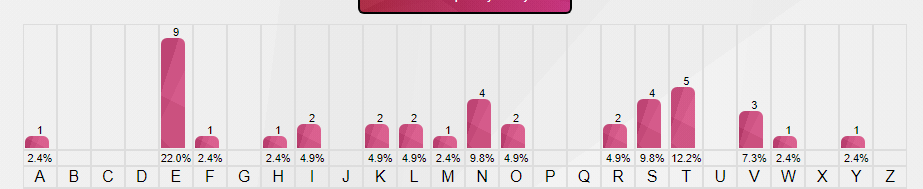
\includegraphics{graph.png} This graph was generated using
https://www.101computing.net/frequency-analysis/.

I have now established that it is probably written in plain englis, we
can then move onto looking for patterns in the text. The thing that
stands out to me is the three e's, they stand out because there is no
word that has three repeating letters in a word. This further pushes me
towards the idea that it is most likely in plain english and it also
makes me wonder if there is some kind of transposition technique
delpoyed. We can also look at pairs of letters, as detailed by Thiagi
group (2015), but this does not yield much as none of the common pairs
seem to be present.

I will now move onto setting up into columns to try to see patterns or
of I can form any words.

SVNYIEAKEEEKLMTRNRHETEETFVTNSLVNIOEESOTWS

SVNYIEAKEEEKLMTRNRHET

EETFVTNSLVNIOEESOTWS

SVNYIEAKEE

EKLMTRNRHET

EETFVTNSLV

NIOEESOTWS

SVNYI

EAKEE

EKLMT

RNRHET

EETFV

TNSLV

NIOEE

SOTWS

Despite finding words like ``seer'' and ``seen'', this does not produce
much of value as it seems like I can't find many more words.

I will now try anagramming to try and find words that make sense. What
makes me curious is the combination ``mtr'' where if you place the most
common letter ``e'' between you get ``meter'', this similarily happens
to ``svn'' which becomes ``seven'' if placed between the letters. Now
looking at the text you can divide it in half and notice a pattern, the
words ``meter'' and ``seven'' are formed if you first first read row one
letter one then row two letter one and so on.

SVNYIEAKEEEKLMTRNRHET EETFVTNSLVNIOEESOTWS

This leads me to believe that it is a rail fence cipher, where the text
is divided into rails and is supposed to be read in order of the rail.
Assuming this is true I will try to form the sentence or word, this
therefore becomes ``SEVENTYFIVETANKSELEVENKILOMETERSNORTHWEST'' using
two rails.

I have therefore concluded that the cipher most likely used is the rail
fence cipher.

Refernce

Frequency analysis. (2022, 2 October) In wikipedia.
https://en.wikipedia.org/wiki/Frequency\_analysis

Thiagi group. (2015, February 15). Cryptograms: New Vision.
http://www.thiagi.com/instructional-puzzles-original/2015/2/13/cryptograms

    \hypertarget{question-7}{%
\subsection{Question 7:}\label{question-7}}

Estimate the amount of time it would take for Python and your personal
computer system to loop through all possible AES-256 keys. Assume that a
new key is updated (saved in a memory location) in each iteration of a
for-loop.

    \begin{tcolorbox}[breakable, size=fbox, boxrule=1pt, pad at break*=1mm,colback=cellbackground, colframe=cellborder]
\prompt{In}{incolor}{1}{\boxspacing}
\begin{Verbatim}[commandchars=\\\{\}]
\PY{k+kn}{import} \PY{n+nn}{time}
\PY{n}{start\PYZus{}time} \PY{o}{=} \PY{n}{time}\PY{o}{.}\PY{n}{time}\PY{p}{(}\PY{p}{)}

\PY{k}{for} \PY{n}{i} \PY{o+ow}{in} \PY{n+nb}{range}\PY{p}{(}\PY{l+m+mi}{110000000}\PY{p}{)}\PY{p}{:}
    \PY{n}{l} \PY{o}{=} \PY{n}{i}
    
\PY{n}{stop\PYZus{}time} \PY{o}{=} \PY{n}{time}\PY{o}{.}\PY{n}{time}\PY{p}{(}\PY{p}{)}
\PY{n+nb}{print}\PY{p}{(}\PY{n}{f}\PY{l+s+s1}{\PYZsq{}}\PY{l+s+s1}{Time taken is }\PY{l+s+s1}{\PYZob{}}\PY{l+s+s1}{stop\PYZus{}time \PYZhy{} start\PYZus{}time\PYZcb{}}\PY{l+s+s1}{\PYZsq{}}\PY{p}{)}
\end{Verbatim}
\end{tcolorbox}

    \begin{Verbatim}[commandchars=\\\{\}]
Time taken is 5.476065158843994
    \end{Verbatim}

    There are \(1,1 * 10^{77}\) different keys in aes 256, I decided to take
out \(1,1 * 10^{8} = 110000000\). If we use this number and run it, it
then takes roughly 5 seconds,if we then make this into years we get
\(\frac{\frac{\frac{\frac{5* 10^{69}}{12}}{60}}{24}}{365} ≈ 8 * 10^{62}\)
years. An unimagineable number.

    \hypertarget{question-8}{%
\subsection{Question 8:}\label{question-8}}

Briefly explain why each of the following statements is true.

\begin{enumerate}
\def\labelenumi{\alph{enumi})}
\tightlist
\item
  \(\gcd(37,36)=37-36\)
\end{enumerate}

    We generalize, \(gcd(x + 1, x) = x + 1 - x\), as we can see
\(x + 1 - x\) will always be equal to \(1\). We let \(x\) and \(x + 1\)
be integers, for any integer that divides both \(x\) and \(x + 1\) this
will also divide \(x - x + 1\). We already concluded that this will
always be equal to \(1\) and the only integer to divide \(1\) is \(1\).
This therefore proves the statement.

Source: https://en.wikipedia.org/wiki/Euclidean\_algorithm

    \begin{enumerate}
\def\labelenumi{\alph{enumi})}
\setcounter{enumi}{1}
\tightlist
\item
  \(256 | 4^{128}\)
\end{enumerate}

    If we have \(n^{x}\) and \(n^{y}\),where \(\frac{n^{y}}{n^{x}}\), then
as long as \(y \geq x\) then it is divisible since it will just be a
multiple of \(n\). For example, \(n = 4\), \(x = 4\) and \(y = 5\), we
can then write \(\frac{4^{5}}{4^{4}} = 4\). Since the base is the same
the numerator will always be a multiple of \(4\).

Working with previous statement we can write \(256\) as \(4^{4}\), which
we plug in \(\frac{4^{128}}{4^{4}}\), this will result in a multiple of
\(4\). This therefore proves the statement.

    \begin{enumerate}
\def\labelenumi{\alph{enumi})}
\setcounter{enumi}{2}
\tightlist
\item
  If \(a\) and \(b\) are prime, then \(c=ab+1\) not necessarily prime.
\end{enumerate}

    If \(a = 3\) and \(b = 5\) then \(3 * 5 + 1 = 16\) which is not a prime.
This example proves then that the statement is true.

    \begin{enumerate}
\def\labelenumi{\alph{enumi})}
\setcounter{enumi}{3}
\tightlist
\item
  If \(p\) is prime and \(a\) is coprime to \(p\), then \(a^{p-1}\) is
  congruent to \(\gcd(a,p)\) modulo \(p\).
\end{enumerate}

    Since \(p\) is prime and \(a\) is coprime to \(p\), that implies that
\(a\) is not divisible by \(p\). We can then use Fermat's theorem which
states that \(a^{p - 1}\) modulo \(p\) is congruent to \(1\). Again
using the fact that \(a\) and \(p\) are coprime, this means that
\(gcd(a, p)\) modulo \(p\) is equal to \$ 1\$. Which means that
\(a^{p - 1} \equiv gcd(a, p)\) can be written as \(1 \equiv 1\),
therefore proving the statement.

    \begin{enumerate}
\def\labelenumi{\alph{enumi})}
\setcounter{enumi}{4}
\tightlist
\item
  \(24 \equiv -51 \mod 5\)
\end{enumerate}

    We find the a property of congruence is that if \(a \equiv b\) modulo
\(n\) if \(n|(a - b)\). If \(a = 24\),\(b = -51\) and \(n = 5\), then
\(5|(24-(-51))\) which can be written as \(\frac{75}{5}=15\). This is is
then true.

    \begin{enumerate}
\def\labelenumi{\alph{enumi})}
\setcounter{enumi}{5}
\tightlist
\item
  \(\phi(\phi(13))=4\)
\end{enumerate}

    The functions works by counting the integer up to a given integer \(x\)
that are relative prime to \(x\). Relative prime is when the only common
divisor is \(1\). We run it through once \(\phi(13) = 12\), this means
that counting from \(1\) to \(13\) there are \(12\) integers that only
have the common divisor of \(1\), \(\phi(12) = 4\) for the same reason.
The answer is therefore 4.

    \hypertarget{question-9}{%
\subsection{Question 9:}\label{question-9}}

For polynomial arithmetic with coefficients in \(\mathbb Z_{11}\),
perform the following calculations. Also, briefly explain the difference
between calculations in \(\mathbb Z_{11}\) and the ``normal'' way
(calculations with coefficients in e.g.~the reals \(\mathbb R\)).

\begin{enumerate}
\def\labelenumi{\alph{enumi})}
\tightlist
\item
  \((x^2 + 2x + 9)(x^3 + 11x^2 + x + 7)\)
\end{enumerate}

    Stallings (2022) explains that polynomial artihmetic with coefficients
\(\mathbb Z_{n}\) is the same as ordinary but that the coefficients
should be in \(\mathbb Z_{n}\). In figure 5.4, it states that
``Arithetmic on coefficients is performed modulo p''. For example
coefficients would therefore be calculated like this \(5 * 5 = 3\) in
\(\mathbb Z_{11}\) since \(5 * 5 = 25\), \(25\) modulo \(11 = 3\). The
difference between how you would normally do it and this way is that
after you have combined equals you would normally not do anything else,
with coefficients in \(\mathbb Z_{11}\) we apply modulo to the
coefficients.

We expand \((x^2 + 2x + 9)(x^3 + 11x^2 + x + 7)\) which results in
\(x^{5}+11x^{4}+x^{3}+7x^{2}+2x^{4}+22x^{3}+2x^{2}+14x+9x^{3}+99x^{2}+0x+63\),
if we then combine equals we get
\(x^{5}+13x^{4}+32x^{3}+108x^{2}+23x+63\). Now we take \((1\) modulo
\(11)x^{5}+(13\) modulo \(11)x^{4}+(32\) modulo \(11)x^{3}+(108\) modulo
\(11)x^{2}+(23\) modulo \(11)x+(63\) modulo
\(11) = x^{5}+2x^{4}+10x^{3}+9x^{2}+x+8\) in \(\mathbb Z_{11}\).

The answer is therfore \(x^{5}+2x^{4}+10x^{3}+9x^{2}+x+8\) in
\(\mathbb Z_{11}\).

Reference

Stallings, W. (2022). Cryptography and Network Security: Principles and
Practice. Pearson.

    \begin{enumerate}
\def\labelenumi{\alph{enumi})}
\setcounter{enumi}{1}
\tightlist
\item
  \((8x^2 + 3x + 2)(5x^2 + 6)\)
\end{enumerate}

    We expand \((8x^{2}+3x+2)(5x^{2}+6)\) which results in
\(40x^{4}+48x^{2}+15x^{3}+18x+10x^{2}+12\), if we then combine equals we
get \(40x^{4}+15x^{3}+58x^{2}+18x+12\). Now we apply modulo 11 to the
coefficients, \((40\) modulo \(11)x^{4}+(15\) modulo \(11)x^{3}+(58\)
modulo \(11)x^{2}+(18\) modulo \(11)x+(30\) modulo
\(11) = 7x^{4}+4x^{3}+3x^{2}+7x+8\).

The answer is therefore \(7x^{4}+4x^{3}+3x^{2}+7x+8\) in
\(\mathbb Z_{11}\).

    \hypertarget{question-10}{%
\subsection{Question 10:}\label{question-10}}

The enemy is poor and can only afford small semiprime RSA moduli
\(n=pq\).

\begin{enumerate}
\def\labelenumi{\alph{enumi})}
\tightlist
\item
  Use Python/Sage to factorize the enemy's modulus
  \(n=2778546901342097\) into its prime factors \(p\) and \(q\), that
  is, find \(p\) and \(q\).
\end{enumerate}

    \begin{tcolorbox}[breakable, size=fbox, boxrule=1pt, pad at break*=1mm,colback=cellbackground, colframe=cellborder]
\prompt{In}{incolor}{65}{\boxspacing}
\begin{Verbatim}[commandchars=\\\{\}]
\PY{k+kn}{from} \PY{n+nn}{math} \PY{k}{import} \PY{n}{sqrt}

\PY{n}{n} \PY{o}{=} \PY{l+m+mi}{2778546901342097}

\PY{k}{def} \PY{n+nf}{factorize}\PY{p}{(}\PY{n}{n}\PY{p}{)}\PY{p}{:}
    \PY{n}{n\PYZus{}original} \PY{o}{=} \PY{n}{n} \PY{c+c1}{\PYZsh{} since n is modified throughtout the code I saved the orgiinal value of in this variable}
    \PY{n}{p} \PY{o}{=} \PY{l+m+mi}{1} 
    \PY{n}{q} \PY{o}{=} \PY{l+m+mi}{1}
    \PY{k}{for} \PY{n}{i} \PY{o+ow}{in} \PY{n+nb}{range}\PY{p}{(}\PY{l+m+mi}{2}\PY{p}{,} \PY{n+nb}{int}\PY{p}{(}\PY{n}{sqrt}\PY{p}{(}\PY{n}{n}\PY{p}{)}\PY{p}{)}\PY{p}{)}\PY{p}{:}
        \PY{k}{if} \PY{n}{n} \PY{o}{\PYZpc{}} \PY{n}{i} \PY{o}{==} \PY{l+m+mi}{0}\PY{p}{:}
            \PY{n}{p} \PY{o}{=} \PY{n}{i}
            \PY{k}{break} \PY{c+c1}{\PYZsh{} for efficieny break when we find it.}

    \PY{n}{q} \PY{o}{=} \PY{n}{n\PYZus{}original} \PY{o}{/}\PY{o}{/} \PY{n}{p}
        
    \PY{k}{return} \PY{n}{p}\PY{p}{,} \PY{n}{q}

\PY{n}{p}\PY{p}{,} \PY{n}{q} \PY{o}{=} \PY{n}{factorize}\PY{p}{(}\PY{n}{n}\PY{p}{)}
\PY{n+nb}{print}\PY{p}{(}\PY{n}{f}\PY{l+s+s1}{\PYZsq{}}\PY{l+s+s1}{P = }\PY{l+s+si}{\PYZob{}p\PYZcb{}}\PY{l+s+s1}{, Q = }\PY{l+s+si}{\PYZob{}q\PYZcb{}}\PY{l+s+s1}{\PYZsq{}}\PY{p}{)}
\end{Verbatim}
\end{tcolorbox}

    \begin{Verbatim}[commandchars=\\\{\}]
P = 15485867, Q = 179424691
    \end{Verbatim}

    Given \(n\) and \(n = pq\), we can then rewrite it as
\(q = \frac{n}{p}\) so the question is then how do we find \(p\). Since
the number is quite small I decided to bruteforce \(p\) and test every
number up to \(\sqrt{n}\) as stated in the thread (Stackoverflow,2011).
Given \(n\) and \(p\) we can then calculate \(q\).

Reference

Stackoverflow. (2011, 27 april). Why do we check up to the square root
of a number to determine if the number is prime?
https://stackoverflow.com/questions/5811151/why-do-we-check-up-to-the-square-root-of-a-number-to-determine-if-the-number-is

    \begin{enumerate}
\def\labelenumi{\alph{enumi})}
\setcounter{enumi}{1}
\tightlist
\item
  Use the \(p\) and \(q\) that you found in a) to find \(\phi(n)\). In
  other words, how can you driectly find \(\phi(n)\) without knowing
  \(n\)?
\end{enumerate}

    \begin{tcolorbox}[breakable, size=fbox, boxrule=1pt, pad at break*=1mm,colback=cellbackground, colframe=cellborder]
\prompt{In}{incolor}{66}{\boxspacing}
\begin{Verbatim}[commandchars=\\\{\}]
\PY{n}{phi\PYZus{}n}\PY{o}{=} \PY{p}{(}\PY{n}{p}\PY{o}{\PYZhy{}}\PY{l+m+mi}{1}\PY{p}{)}\PY{o}{*}\PY{p}{(}\PY{n}{q}\PY{o}{\PYZhy{}}\PY{l+m+mi}{1}\PY{p}{)}
\PY{n+nb}{print}\PY{p}{(}\PY{n}{phi\PYZus{}n}\PY{p}{)}
\end{Verbatim}
\end{tcolorbox}

    \begin{Verbatim}[commandchars=\\\{\}]
2778546706431540
    \end{Verbatim}

    Stallings (2022) figure 9.5 states that ``\(\phi(n)=(p-1)(q-1)\)'', also
referenced in (``RSA (cryptosystem)'', 2022), this means that given
\(q\) and \(p\) we can calculate \(\phi(n)\).

Reference

Stallings, W. (2022). Cryptography and Network Security: Principles and
Practice. Pearson.

RSA (cryptosystem). (2022, 16 October) In wikipedia.
https://en.wikipedia.org/wiki/RSA\_(cryptosystem)

    \begin{enumerate}
\def\labelenumi{\alph{enumi})}
\setcounter{enumi}{2}
\tightlist
\item
  The enemy seems to be using the RSA modulus \(n=2778546901342097\) as
  in a) above and the public exponent \(e=65537\). Use the Extended
  Euclidean algorithm to find the private exponent \(d\). You can use
  e.g.~the built-in Sage function for the Extended Euclidean algorithm.
\end{enumerate}

    \begin{tcolorbox}[breakable, size=fbox, boxrule=1pt, pad at break*=1mm,colback=cellbackground, colframe=cellborder]
\prompt{In}{incolor}{67}{\boxspacing}
\begin{Verbatim}[commandchars=\\\{\}]
\PY{n}{e} \PY{o}{=} \PY{l+m+mi}{65537}
\PY{n}{coprime} \PY{o}{=} \PY{n}{gcd}\PY{p}{(}\PY{n}{e}\PY{p}{,}\PY{n}{phi\PYZus{}n}\PY{p}{)}
\PY{n+nb}{print}\PY{p}{(}\PY{n}{f}\PY{l+s+s1}{\PYZsq{}}\PY{l+s+s1}{Coprime check for E and φ(n), value = }\PY{l+s+si}{\PYZob{}coprime\PYZcb{}}\PY{l+s+s1}{\PYZsq{}}\PY{p}{)}

\PY{n}{e} \PY{o}{=} \PY{l+m+mi}{65537}
\PY{n}{d} \PY{o}{=} \PY{n}{xgcd}\PY{p}{(}\PY{n}{e}\PY{p}{,}\PY{l+m+mi}{2778546706431540}\PY{p}{)}
\PY{n}{d} \PY{o}{=} \PY{n}{d}\PY{p}{[}\PY{l+m+mi}{1}\PY{p}{]}
\PY{n+nb}{print}\PY{p}{(}\PY{n}{d}\PY{p}{)}
\end{Verbatim}
\end{tcolorbox}

    \begin{Verbatim}[commandchars=\\\{\}]
Coprime check for E and φ(n), value = 1
1330108882324133
    \end{Verbatim}

    Similar to before where the book (Stallings, 2022) figure 9.5 defines
\(d = e^{-1}(\) mod \(φ(n))\). Where \(e^{-1}\) is the multiplicative
inverse, according to ``Extended Euclidean algorithm'' (2022) already
does this which is why it is used.

Reference

Stallings, W. (2022). Cryptography and Network Security: Principles and
Practice. Pearson. Extended Euclidean algorithm. (2022, 30 September) In
wikipedia. https://en.wikipedia.org/wiki/Extended\_Euclidean\_algorithm

    \begin{enumerate}
\def\labelenumi{\alph{enumi})}
\setcounter{enumi}{3}
\tightlist
\item
  Based on the the information you have found so far, decrypt
  \(319111435225580\).
\end{enumerate}

    \begin{tcolorbox}[breakable, size=fbox, boxrule=1pt, pad at break*=1mm,colback=cellbackground, colframe=cellborder]
\prompt{In}{incolor}{68}{\boxspacing}
\begin{Verbatim}[commandchars=\\\{\}]
\PY{k+kn}{from} \PY{n+nn}{builtins} \PY{k}{import} \PY{n+nb}{pow} \PY{c+c1}{\PYZsh{} because sagemath overrides the pow function and I need the funtionality of the built\PYZhy{}in version}
\PY{n}{C} \PY{o}{=} \PY{l+m+mi}{319111435225580}

\PY{n}{decrypted} \PY{o}{=} \PY{n+nb}{pow}\PY{p}{(}\PY{n}{C}\PY{p}{,}\PY{n}{d}\PY{p}{,}\PY{n}{n}\PY{p}{)}
\PY{n+nb}{print}\PY{p}{(}\PY{n}{decrypted}\PY{p}{)}
\end{Verbatim}
\end{tcolorbox}

    \begin{Verbatim}[commandchars=\\\{\}]
12345
    \end{Verbatim}

    Taken from the book (Stallings, 2022) figure 9.5 \(M = C^{d}\) mod
\(n\). We simply plug in the variables and get the decrypted message.

Reference

Stallings, W. (2022). Cryptography and Network Security: Principles and
Practice. Pearson.

    \hypertarget{question-11}{%
\subsection{Question 11:}\label{question-11}}

Encrypt the phrase ``jamesbondliveandletdie'' (just like in question 5)
with the Playfair cipher but now use your first name as the keyword. You
can choose I/J by yourself if needed. First give your first name that
you use as the keyword so that we can check that the solution is
correct.

Your name/keyword: MIKAEL

    Since this question is so similar to the last one I will work from that
reference and the explanation given there.

We first generate the square
\(\begin{matrix}M & I & K & A & E\\L & B & C & D & F\\G & H & N & O & P\\Q & R & S & T & U\\V & W & X & Y & Z\\\end{matrix}\).
We get the pairs from last time ``ja'' ``me'' ``sb'' ``on'' ``dl''
``iv'' ``ea'' ``nd'' ``le'' ``td'' ``ie''.

pair - encrypted pair

ja - ke

me - im

sb - rc

on - po

dl - fb

iv - mw

ea - me

nd - oc

le - fm

td - yo

ie - km

The final encrypted text is ``keimrcpofbmwmeocfmyokm''.

    \hypertarget{question-12}{%
\subsection{Question 12:}\label{question-12}}

(essay, max length 2.5 pages including figures)

The following people are famous figures in the history of cryptography.
Write a short biography on one the people. Especially explain what
contributions the person (has) made to cryptography. Focus mostly on the
concepts and terminology used on our course.

\begin{itemize}
\tightlist
\item
  Boris Hagelin
\item
  Auguste Kerckhoffs
\item
  Ralph Merkle
\item
  Claude Shannon
\item
  Alan Turing
\end{itemize}

Essay title: Alan Turing

    \hypertarget{alan-turings-contributions-to-cryptography-and-cryptanalysis}{%
\subsection{Alan Turing's contributions to cryptography and
cryptanalysis}\label{alan-turings-contributions-to-cryptography-and-cryptanalysis}}

Alan Turing, regarded as the ``father of modern computing'' (Tucker,
2022), was a British mathematician who contributed immensely to the
fields of mathematics and cryptanalysis and helped create the foundation
for fields like computer science and artificial intelligence. In the
second world war, Turing played an integral part in breaking the enigma
machine which was used by the Germans to encrypt messages. For this he
was later awarded by being given the title of OBE. An award given to
people for being known nationally in a field of expertise (Gov.uk,
n.d.). His contributions to computing were significant as Turing created
and input-output system, programming system and a programming manual for
the first marketable electronic computer (Copeland, 2022). This essay
will focus on his contributions to the field of cryptography, more
specifically cryptanalysis.

The enigma machine was a device that utilized a substitution cipher to
encrypt commercial, diplomatic and military communications. The machine
was capable of both encryption and decryption if they have the same key,
which in this case is the same as the machine settings. This would
therefore qualify as symmetric encryption; security was provided by
changing the machine settings regularly. This means that the machine
that is decrypting a message must be configured the same as the machine
was that encrypted it (``Enigma machine'', 2022). Turing and Gordon
Welchman developed a machine called Bombe, which was used to break
Enigma-enciphered messages during the second world war. Since the
Germans were changing settings daily, it was integral to find out what
these settings were so that the messages could be deciphered in time.
The machine allowed the British to find the key, which is the settings
for the machine, within hours of receiving a message (The national
computing of computing, n.d.).

The word ``cribs'' is used to describe any known or suspected plaintext
that is commonly occurring. One attack vector is therefore a known
plaintext-attack, where the attacker knows part of the words, in the
plaintext, or the whole plaintext. This was used by the cryptanalysts,
which Turing was amongst, to break the Enigma. They realized that the
Germans would regularly send weather reports and a commonly used phrase
was ``Nothing to report'' (101 computing, 2019). Once a crib had been
found they were able to brute force the key using Bombe, this
combination of developing Bombe and the usage of cribs was largely
attributed to Turing. Bombe acted like 36 Enigma machines and went
through every possible setting, every combination was checked using the
Bombe's comparator unit and if no logical contradiction was found, then
those settings were written down as a potential candidate (Ludlow,
2019).

Turingery, also called Turing's method, was a method developed by Turing
which made it possible to figure out how a cipher machine was
constructed using the keys used to encrypt and decrypt messages
(``Turingery'', 2022). This method was utilized in breaking the SZ40,
the Lorenz SZ40 was a German developed rotor stream cipher machine that
was used by Germany during the second world war, Lorenz was used for
transmitting at the highest level of German command (``Lorenz cipher'',
2022). The Lorenz machine utilized a much more sophisticated cipher and
was a lot harder to break, William Tutte managed to figure out the inner
workings of the machine without ever seeing it. Sometimes two messages
would be transmitted using the same key, it was therefore possible to
extract the keys and use that to figure out how the machine worked. This
is due to the Turingery method (Zitarelli, 2015).

Cryptography goes back to ancient times, but it has evolved especially
in the modern age with the computational power we have today. What might
have taken days could be brute forced in minutes. This can be attributed
to Turing's contribution as he laid the foundation for computing and
allowed everyone to have the power of a computer (Tresorit team, 2022).
This pushed cryptography to become more advanced as computers were
sophisticated enough and powerful enough to brute force and perform
calculations much faster than a human. Turing published a paper titled
``can machines think?'' in 1950, he detailed a way to test if a machine
is truly thinking called the ``Turing test''. Turing, along with Alonzo
Chruch, came up with the Church-Turing thesis which states that there
are mathematical problems that can't be computed (Aron, J; n.d.). This
essentially means there's a limit to computational power (L. Casti,
Calude, n.d.).

Despite these contributions to the scientific field of mathematics,
cryptanalysis and creating the foundation for computer science, and his
great contributions to the war effort through breaking the Enigma,
Turing met an early end as in 1952 he was convicted for being a
homosexual and was sentenced to be undergo hormone treatment for 12
months. In 1954 he was found dead; the official cause of death was ruled
a suicide by cyanide poisoning. He broke the Enigma, and he devised a
method that broke the Lorenz machine, saving countless of lives in the
process. In 2013 Turing was pardoned and in 2019 he was voted the
``greatest person of the 20th century'', that is the legacy of Alan
Turing and his impact on cryptography and the world. (``Alan Turing,
2022'').

Reference list

  Tucker, A. (2022, August 24). Computer science. Encyclopedia
Britannica. https://www.britannica.com/science/computer-science

Gov.uk. (n.d.). Nominate someone for an honour or award.
https://www.gov.uk/honours/types-of-honours-and-awards

Copeland, B. (2022, August 12). Alan Turing. Encyclopedia Britannica.
https://www.britannica.com/biography/Alan-Turing

Wikipedia contributors. (2022, October 22). Enigma machine. In
Wikipedia, The Free Encyclopedia. Retrieved 17:34, October 21, 2022,
from
https://en.wikipedia.org/w/index.php?title=Enigma\_machine\&oldid=1117498764

The national museum of computing. (n.d.). The Turing-Welchman Bombe.
https://www.tnmoc.org/bombe

101 computing. (2019, May 9). Enigma Crib Analysis.
https://www.101computing.net/enigma-crib-analysis/

Ludlow, D. (2011, January 20). How Bletchley Park broke the German
Enigma code.
https://www.expertreviews.co.uk/technology/7857/how-bletchley-park-broke-the-german-enigma-code

Wikipedia contributors. (2022, January 5). Turingery. In Wikipedia, The
Free Encyclopedia. Retrieved 18:43, October 22, 2022, from
https://en.wikipedia.org/w/index.php?title=Turingery\&oldid=1063877878

Wikipedia contributors. (2022, April 10). Lorenz cipher. In Wikipedia,
The Free Encyclopedia. Retrieved 18:59, October 22, 2022, from
https://en.wikipedia.org/w/index.php?title=Lorenz\_cipher\&oldid=1081881709

Zitarelli, D. (2015, January). Alan Turing in America -- Cryptography.
https://www.maa.org/press/periodicals/convergence/alan-turing-in-america-cryptography

Tresorit team. (2022, January 14). The history of encryption: the roots
of modern-day cyber-security.
https://tresorit.com/blog/the-history-of-encryption-the-roots-of-modern-day-cyber-security/

Aron, J. (n.d.) Alan Turing.
https://www.newscientist.com/people/alan-turing/

L. Casti, J, Calude, C. (n.d.). The jumble cruncher.
https://www.newscientist.com/article/mg18324665-500-the-jumble-cruncher/

Wikipedia contributors. (2022, October 23). Alan Turing. In Wikipedia,
The Free Encyclopedia. Retrieved 19:28, October 22, 2022, from
https://en.wikipedia.org/w/index.php?title=Alan\_Turing\&oldid=1117844782

    \hypertarget{questions-13-to-24-are-short-questions-that-must-be-answered-with-just-a-couple-of-sentences-with-or-without-a-single-optional-figure.-references-are-not-required-for-these-answers.-be-concise-and-on-point.}{%
\subsection{Questions 13 to 24 are ``short questions'' that must be
answered with just a couple of sentences with or without a single
optional figure. References are not required for these answers. Be
concise and on
point.}\label{questions-13-to-24-are-short-questions-that-must-be-answered-with-just-a-couple-of-sentences-with-or-without-a-single-optional-figure.-references-are-not-required-for-these-answers.-be-concise-and-on-point.}}

    \hypertarget{question-13}{%
\subsection{Question 13:}\label{question-13}}

(short question)

Explain the PGP architecture. What does it have to do with symmetric and
asymmetric encryption?

    PGP encryption follows a couple of steps, first the plaintext is
compressed. A randomly generated key is then generated to encrypt the
plaintext, this key is later encrypted using a public key. The reason
why this is interesting is because it is both symmetric and asymmetric
in the sense that encrypting the plaintext is done symmetrically and the
encryption of the key is done asymmertically.

    \hypertarget{question-14}{%
\subsection{Question 14:}\label{question-14}}

(short question)

Briefly explain the Diffie-Hellman key exchange procedure. Also explain
why it is such a popular and convenient system.

    The DH key exchange works by using a common public key and each party
having a private key that can be anything. Each party will use their
private key and apply it to the public key to produce the mixed key, the
mixed key is then exchanged and they apply their private key again. The
two parties should now have the same key which they can use to encrypt
and decrypt messages between eachother. Even if someone listens to the
exchange of keys they can only get the mixed keys and the common public
key and from this information it can be very hard to figure out the
private keys. The reason for why it's a popular system is because the
two parties can now send encrypted messages and it is not easy to get
the key to decrypt those messages. The convenience comes from the
relative simplicity, all that is needed is a common public key and for
each party to generate their own key.

    \hypertarget{question-15}{%
\subsection{Question 15:}\label{question-15}}

(short question)

What is a backdoor to a cryptosystem? Do you believe backdoors to
systems like AES, DES and RSA are likely?

    A backdoor would be a way to go around encryption and gain access to the
encrypted data, these backdoors are deliberately created for various
reasons such as giving a select few people the ability to decrypt
messages when it relates to crime. An example of a backdoor would be a
universal key that can decrypt every message. While backdoors can be
useful they do pose a security risk and that's why I believe that AES,
DES and RSA do not have any backdoors, these are three are huge
algorithms that are trusted to be safe and that's why I believe they
don't.

    \hypertarget{question-16}{%
\subsection{Question 16:}\label{question-16}}

(short question)

What are digital signatures and message authentication codes? What are
the major differences between the two?

    They are both ways to ensure the integrity of dat aand its authenticity,
they both work similarily. The major differences are non-repudiation and
public/private keys. Message authentication codes are generated using
the same secret key, while digital signatures uses both public and
private keys. Digital signatures provide non-repudiation (ensures
integrity and origin of data) since the private key is only known by the
holder. The message authentication codes both use the same key which
means that anyone with the key can produce a code for any message.

    \hypertarget{question-17}{%
\subsection{Question 17:}\label{question-17}}

(short question)

What is a side-channel attack? What can you do to prevent side-channel
attacks?

    A side-channel attack is an attack based on information that is
physicall leaked through the use of a cryptosystem. These can include
checking how much power is used by the system or the sound that is made
from various pieces of hardware. Side-channel attacks can rely on a lot
of information that is leaked, if you want to prevent these you will
want to make sure that the system leaks as little information as it can.
To counter acoustic attacks, installing acoustic shielding foam to
reduce the amount of sound that leaks could be one option, another could
be to make sure that the cryptosystem is far away from people.

    \hypertarget{question-18}{%
\subsection{Question 18:}\label{question-18}}

(short question)

What is a replay attack? What can you do to prevent replay attacks?

    A replay attack is where an attacker either replays or delays a message.
Some form of authentification of the messages like adding timestaps or
the use of one-time passwords.

    \hypertarget{question-19}{%
\subsection{Question 19:}\label{question-19}}

(short question)

What is a known-plaintext attack? Why are substitution ciphers
vulnerable to known-plaintext attacks?

    A known-paintext attack is an attack where the attacker has both the
paintext and the ciphertext. The reason why substituion ciphers are so
weak to this attack is that you can map out which letter substitutes
which, popular example of this is the enigma where every message ended
with a phrase ``HH''(not writing it out to avoid trouble).

    \hypertarget{question-20}{%
\subsection{Question 20:}\label{question-20}}

(short question)

What is the difference between differential and linear cryptanalysis?

    Differential cryptanalysis studies how changes in the plaintext affects
the ciphertext. Linear cryptanylsis studies the bits of the plaintext,
the ciphertext and the unknown key to find linear relationships.

    \hypertarget{question-21}{%
\subsection{Question 21:}\label{question-21}}

(short question)

What is the Kerchoff's principle? Why should we follow this principle?

    Kerchoff's principle says that a system should be secure even if
everything about the system is, except the key, is publicly known. One
of the reasons why this principle is good to follow is because it is
easier to maintain the security of the system, if an intruder manages to
get their hands on the key, then instead of changing major parts of the
system you can just change the key. The key is another big reason as to
why this principle is good, the less you need to keep secret the easier
it would hopefully be. So instead of having to keep major parts of a
system secret you only need to keep the key a secret.

    \hypertarget{question-22}{%
\subsection{Question 22:}\label{question-22}}

(short question)

What are TRNGs and PRNGs? Give one or more examples of each.

    TRNG tsands for true random number generator while PRNG stands for
pseudorandom number generator. TRNG can be provided by dedicated
hardware that uses a physical process instead of an algorithm to
generate random numbers. PRNG is an algorithm that generates a sequence
of numbers that have similar properties to sequences of random numbers,
this makes them not truly random and only somewhat like random numbers.
It is even possible to predict these ``random'' numbers in python.

    \hypertarget{question-23}{%
\subsection{Question 23:}\label{question-23}}

(short question)

What is the main drawback of RSA compared to ECC (elliptic curve
cryptography)?

    ECC can give the same security as RSA with smaller keys, smaller keys
requires less computational power and less load for the network.

    \hypertarget{question-24}{%
\subsection{Question 24:}\label{question-24}}

(short question)

What is the man-in-the-middle attack on the Diffie-Hellman protocol?
What can be done to thwart this attack?

    When A interecepts B's mixed key(the combination of the common key and
secret key), A can then send their own mixed key to C and then gets C's
mixed key back. A and B then agree on a shared key and B and C agree on
another key. Now whenever B sends a message to C, A has to decrypt and
encrypt every message sent between the two. A way to thwart this attack
is to provide some form of authentification.


    % Add a bibliography block to the postdoc
    
    
    
\end{document}
